\documentclass[10pt, mathserif]{beamer}

\usepackage{listings}
\usepackage{color}
\usepackage{amssymb, amsmath}
\usepackage[all]{xy}
\usepackage{alltt}
\usepackage{pslatex}
\usepackage{epigraph}
\usepackage{verbatim}
\usepackage{graphicx}
\usepackage{latexsym}
\usepackage{array}

\makeatletter
\newcolumntype{e}[1]{%--- Enumerated cells ---
   >{\minipage[t]{\linewidth}%
     \NoHyper%                Hyperref adds a vertical space
     \let\\\tabularnewline
     \enumerate
        \addtolength{\rightskip}{0pt plus 50pt}% for raggedright
        \setlength{\itemsep}{-\parsep}}%
   p{#1}%
   <{\@finalstrut\@arstrutbox\endenumerate
     \endNoHyper
     \endminipage}}

\newcolumntype{i}[1]{%--- Itemized cells ---
   >{\minipage[t]{\linewidth}%
        \let\\\tabularnewline
        \itemize
           \addtolength{\rightskip}{0pt plus 50pt}%
           \setlength{\itemsep}{-\parsep}}%
   p{#1}%
   <{\@finalstrut\@arstrutbox\enditemize\endminipage}}

\AtBeginDocument{%
    \@ifpackageloaded{hyperref}{}%
        {\let\NoHyper\relax\let\endNoHyper\relax}}
\makeatother

\definecolor{shadecolor}{gray}{1.00}
\definecolor{darkgray}{gray}{0.30}

\newcommand{\set}[1]{\{#1\}}
\newcommand{\angled}[1]{\langle {#1} \rangle}
\newcommand{\fib}{\rightarrow_{\mathit{fib}}}
\newcommand{\fibm}{\Rightarrow_{\mathit{fib}}}
\newcommand{\oo}[1]{{#1}^o}
\newcommand{\inml}[1]{\mbox{\lstinline{#1}}}

\setlength{\epigraphwidth}{.55\textwidth}

\definecolor{light-gray}{gray}{0.90}
\newcommand{\graybox}[1]{\colorbox{light-gray}{#1}}

\newcommand{\nredrule}[3]{
  \begin{array}{cl}
    \textsf{[{#1}]}& 
    \begin{array}{c}
      #2 \\
      \hline
      \raisebox{-1pt}{\ensuremath{#3}}
    \end{array}
  \end{array}}

\newcommand{\naxiom}[2]{
  \begin{array}{cl}
    \textsf{[{#1}]} & \raisebox{-1pt}{\ensuremath{#2}}
  \end{array}}

\lstdefinelanguage{ocaml}{
keywords={let, begin, end, in, match, type, and, fun, 
function, try, with, class, object, method, of, rec, repeat, until,
while, not, do, done, as, val, inherit, module, sig, @type, struct, 
if, then, else, open, virtual, new, fresh},
sensitive=true,
basicstyle=\small,
commentstyle=\scriptsize\rmfamily,
keywordstyle=\ttfamily\bfseries,
identifierstyle=\ttfamily,
basewidth={0.5em,0.5em},
columns=fixed,
fontadjust=true,
literate={->}{{$\to$}}1
         {===}{{$\equiv$}}1
}

\lstdefinelanguage{scheme}{
keywords={define, conde, fresh},
sensitive=true,
basicstyle=\small,
commentstyle=\scriptsize\rmfamily,
keywordstyle=\ttfamily\bfseries,
identifierstyle=\ttfamily,
basewidth={0.5em,0.5em},
columns=fixed,
fontadjust=true,
literate={==}{{$\equiv$}}1
}

\lstset{
basicstyle=\small,
identifierstyle=\ttfamily,
keywordstyle=\bfseries,
commentstyle=\scriptsize\rmfamily,
basewidth={0.5em,0.5em},
fontadjust=true,
escapechar=!,
language=ocaml
}

\setbeamertemplate{footline}[frame number]
\setbeamertemplate{navigation symbols}{}
\setbeamertemplate{blocks}[rounded][shadow=true] 
\beamertemplateballitem

\mode<presentation>{
  \usetheme{default}
}

\theoremstyle{definition}

\title{Typed Embedding of a Relational Language in OCaml}

\author[Dmitrii Kosarev, Dmitrii Boulytchev]{\underline{Dmitrii Kosarev}, Dmitrii Boulytchev}

\institute[]{
\small{
\textbf{Saint-Petersburg State University} \\
\textbf{JetBrains Research}
}
}

\date{
   \vskip 1cm
   \small{
   \textbf{ML Family Workshop}\\
   September 22, 2016 \\
   Nara, Japan}
}

\begin{document}
\begin{frame} 
  \titlepage
\end{frame}

\begin{frame}{Relational Programming in miniKanren}
 \vskip1cm
 \begin{center}
 From programs as \emph{functions} to programs as \emph{relations}: 
 \end{center}
 
 $$
 f \colon X \to Y\;\leadsto\;\oo{f} \subseteq X\times Y
 $$
 \vskip5mm
 \begin{tabular}{m{4cm}m{6cm}}
    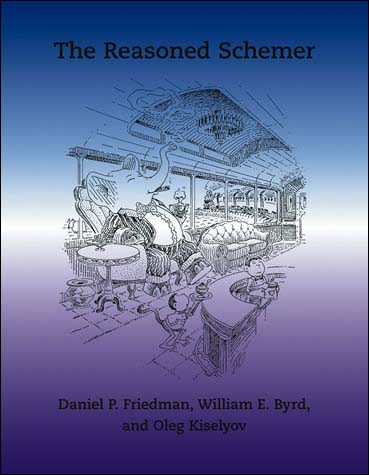
\includegraphics[scale=0.3]{trs.jpg} &
    \begin{itemize} 
       \item Daniel P. Friedman, William Byrd and Oleg Kiselyov. \emph{The Reasoned Schemer}, 
             The MIT Press, Cambridge, MA, 2005    
       \item A DSL for Scheme/Racket with rather simple minimal implementation 
       \item A family of languages ($\mu$Kanren, $\alpha$-Kanren, cKanren etc.)
       \item Implemented as DSL for a wide range of host languages (including OCaml, Haskell, Scala etc.)  
    \end{itemize}   
 \end{tabular}
 \vskip 3cm
\end{frame}

\begin{frame}[fragile]{An Example: Relational List Append}
\vskip5mm
\begin{tabular}{m{5cm}m{5cm}}
 \graybox{$\inml{append} \colon \alpha\:\inml{list} \to \alpha\:\inml{list} \to \alpha\:\inml{list}$} &
 \graybox{$\oo{\inml{append}} \subseteq \alpha\:\inml{list} \times \alpha\:\inml{list} \times \alpha\:\inml{list}$}\\
 \begin{lstlisting}[language=ocaml] 
!\pause!let rec append xs ys!\pause! = 
  match xs with!\pause!
  | []    ->  ys!\pause!
  | h::tl ->  h :: (append tl ys)!\pause!
 \end{lstlisting} &
 \begin{lstlisting}[mathescape=true,language=ocaml]
let rec append$^o$ xs ys xys!\pause! = 
  ((xs === nil) &&& (xys === ys))!\pause! |||  
  (fresh (h t tys)!\pause!
     (xs  === h % t)!\pause! 
     (xys === h % tys)!\pause!
     (append$^o$ t ys tys)
  ) 
 \end{lstlisting}
\end{tabular}\pause
\begin{center}
\begin{minipage}{6cm}
\begin{lstlisting}[mathescape=true,language=scheme]
(define (append$^o$ xs ys xys) 
   (conde 
      [(== '() xs) (== ys xys)]
      [(fresh (h t tys)
         (== `(,h . ,t) xs)
         (== `(,h . ,tys) xys)
         (append$^o$ t ys tys))]))
\end{lstlisting}
\end{minipage}
\end{center}
\vskip5mm
\end{frame}

\begin{frame}[fragile]{Implementation Sketch}
Jason Hemann, Daniel P. Friedman. \emph{$\mu$Kanren: A Minimal Functional 
Core for Relational Programming} // Scheme'13:

\begin{itemize}
\item Logic variables: $X=\{x_1,x_2,\dots\}$;
\item Symbols (constructors): $S=\{s_1,s_2,\dots\}$;
\item Terms: $T=X\cup\{s\;(t_1,\dots,t_k)\mid s\in S,\; t_i \in T\}$;
\item Substitutions: $\Sigma=T^X$;
\item Unification: $(\equiv) \colon \Sigma \to T \to T \to \Sigma_\perp$;
\item State: a substitution + some info to create fresh variables;
\item Goal: 
\end{itemize}

\end{frame}

\begin{frame}[fragile]{Current Implementation}

\begin{itemize}
\item Repository: \url{https://github.com/dboulytchev/OCanren}
\item Implements $\mu$Kanren + disequality constraints
\item Passes most of the orignal tests
\item Outperforms $\mu$Kanren on long queries
\end{itemize}

\end{frame}

\end{document}
